\svnid{$Id: daten.tex 108 2012-05-12 18:44:01Z dgens001 $}
\chapter{Daten- und Domänenmodell}
\textit{In diesem Kapitel bemühen wir uns um eine formale Darstellung der Gegenstandswelt der Anwendung. Es 
werden die Objekthierarchie und die wichtigsten Konzepte, die in der \gls{Welt} auftauchen, beschrieben.}

\section{Überblick}
Im \gls{Spiel} gibt es \glspl{GameObject} und einen \gls{Campus} (später eventuell mehrere). 
Der \gls{Campus} besteht aus \glspl{Raum}n, die wiederum aus \glspl{Feld}n bestehen. Ein \gls{Feld} kann eine 
feste Anzahl an \glspl{GameObject} aufnehmen. Im \gls{Spiel} tauchen verschiedene \glspl{GameObject} auf, z.B. 
\glspl{Charakter}, \glspl{Objekt} oder \glspl{Gegenstand}. Sowohl der \gls{Spieler} als auch \gls{npcs} sind
\glspl{Charakter}. 
Das Spiel ist gewonnen, sobald die Gewinnbedingung erfüllt wurde. Die Gewinnbedingung besteht darin einen 
bestimmten \gls{Schein} zu erlangen. Ein \gls{Spiel} kann neu gestartet, abgespeichert oder geladen werden.
Das Ziel des \gls{Spiel}s könnte später auch durch einen Abschluss 
repräsentiert werden. Der Abschluss würde sich beispielsweise immer aus sechs Semestern zusammensetzen
und diese würden wiederum aus mehreren \glspl{Schein}n bestehen.

\section{Objekte und Gegenstände}
Grundsätzlich gibt es \glspl{Objekt} und \glspl{Gegenstand}. Objekte sind stationäre Gebilde auf einem Feld,
die der Spieler nicht mitnehmen kann. \glspl{Gegenstand} dagegen sind portabel, der Spieler kann sie in sein
Inventar packen. Auch NPCs können Gegenstände mit sich tragen. Häufig auftauchende Gegenstände sind zum 
Beispiel \glspl{Item}. Der Spieler soll mit jeder Form von Gegenstand und den meisten Objekte interagieren
können. Die Reaktion der Gegenstände auf bestimmte Interaktionen kann intern durch einfaches Nachschauen in
einer Tabelle geschehen. Jeder Gegenstand kann dann eine oder mehrere besondere Formen und eine standardmäßige
Form von Interaktion haben um alle Kombinationen möglichst einfach abdecken zu können.
In folgendem UML-Diagramm wird die Domainstruktur bildlich dargestellt. Die grünen Klassen zeigen mögliche 
spätere Erweiterungen an. Sie werden hier nur zur Orientierung abgebildet und sind nicht Teil der 
Spezifikation.
\newpage
\begin{figure}[htb]
	\begin{center}
		%trim option's parameter order: left bottom right top
		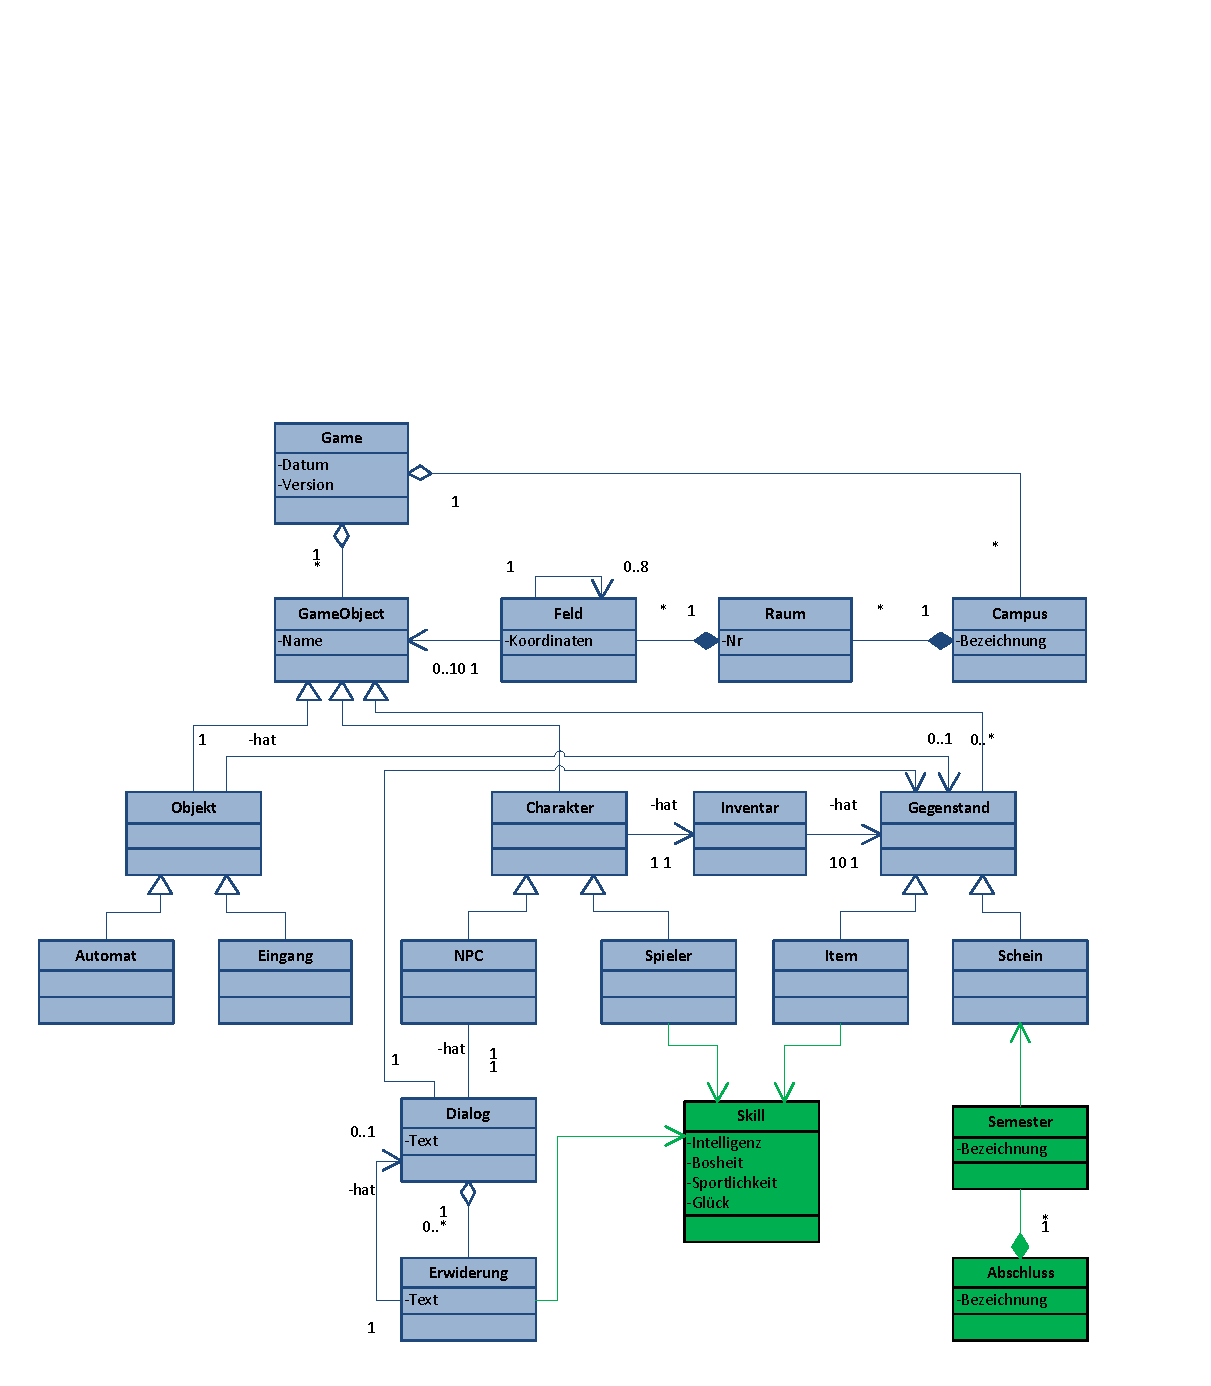
\includegraphics[trim = 5mm 5mm 20mm 40mm, clip, width=14cm]{kapitel/daten/domain.pdf}
	\end{center}
	\caption{UML-Diagramm der Domain}
	\label{fig:domain_uml}
\end{figure}

\newpage
\section{Inventar}
Das Inventar bietet dem \gls{Spieler} die Möglichkeit \glspl{Item} in seinen Besitz zu bringen. Es beinhaltet
eine feste Anzahl an Slots. Jeder Slot kann mit nur einem \gls{Item} belegt werden. Die Anzahl der Items im
Besitz des Spielers ist also durch die Kapazität des Inventars (plus eins im Handslot) direkt beschränkt.
Der Spieler kann Items aus dem Inventar ablegen (droppen) oder in die Hand nehmen (benutzen). Auch NPCs können
ein Inventar haben und Gegenstände mit sich herumtragen. Der Spieler kann Items also nicht nur durch das
Aufnehmen von Feldern, sondern auch durch die Interaktion (z.B. den Dialog) mit NPCs erlangen.

\section{Felder, Räume und Campi}
Felder sind die kleinste räumliche (ebene) Einheit im Spiel. Felder haben eine feste Anzahl Slots (eine 
Quadratzahl, in unserem Spiel neun) und können maximal Slots + 1 viele Elemente aufnehmen (der Spieler muss 
immer auf ein Feld
navigieren können, auch wenn alle Slots belegt sind). Jedes Feld hat kein bis maximal acht
angrenzende Felder. Felder haben Koordinaten. Der Übergang zwischen zwei Feldern muss nicht immer möglich
sein, so können diese durch eine Wand getrennt sein, was dem Spieler ersichtlich sein sollte.
Der Spieler steht immer genau auf einem Feld und kann alle unmittelbar angrenzenden Felder in Blickrichtung
sehen (aber 
nicht notwendigerweise erreichen oder betreten). Auf diesem Feld hat er eine von genau vier 
Blickrichtungen. Diese werden mit N, S, O, W bezeichnet. Diagonal angrenzende Felder kann er gegebenenfalls
sehen, jedoch nicht direkt betreten oder darauf zugreifen.
Räume bestehen aus zusammenhängenden Feldern, die einander zugänglich und vom Rest des \gls{Campus} durch
Wände abgetrennt sind. Räume sind mit einander durch Eingänge verbunden. Eingänge können verschlossen oder
offen sein. Eingänge können auch mit Items (z.B. Schlüsseln) kombiniert werden. Alle Räume zusammen bilden
einen Campus. In der vorgelegten Version spezifizieren wir genau einen Campus pro Spiel.

\section{NPCs und Dialoge}
NPCs sind Nichtspielercharaktere, die auf einem Feld stehen. Der Spieler kann mit ihnen in Form von Dialogen
oder durch Items interagieren. Dialoge haben keine oder mehrere Erwiderungen, die der Spieler dem NPC geben
kann. Eine Erwiderung kann einen Folgedialog haben. Dialoge werden also in Form eines Baums repräsentiert,
in der es einen Einstiegsdialog (Vaterknoten) mit Erwiderungen (den Pfaden) und Folgedialogen (Kindknoten)
geben kann. Manche Dialoge können Gegenstände enthalten, der Spieler erhält also den Gegenstand, vorausgesetzt
er wählt die richtige Abfolge von Erwiderungen. NPCs sollen stationär sein, in späteren Erweiterungen könnten
sich NPCs aber auch auf festen Routen durch die Map von Feld zu Feld bewegen.

\section{Spieler und Scheine}
In der hier vorgelegten Version gibt es nur einen Schein, den es zu finden gilt. Sobald der Schein gefunden
wurde, ist das Spiel automatisch beendet. In zukünftigen Erweiterungen könnten \glspl{Schein} dem 
\gls{Spieler} CPs einbringen. Das Finden der \glspl{Schein} könnte dann an eine Reihe von inhaltlichen
Verpflichtungen geknüpft sein (z.B. "finde \gls{Item} A, damit dir NPC B Schein C überreicht"). Das Ganze
könnte dann in Form von Semestern und Abschlüssen weiter ausgebaut werden, wie schon zuvor angedeutet.

